%%%%%%%%%%%%%%%%%%%% Cover page %%%%%%%%%%%%%%%%%%%%
\begin{center}
~\vspace{4cm}\newline
{\Huge{Задачник.NET}}
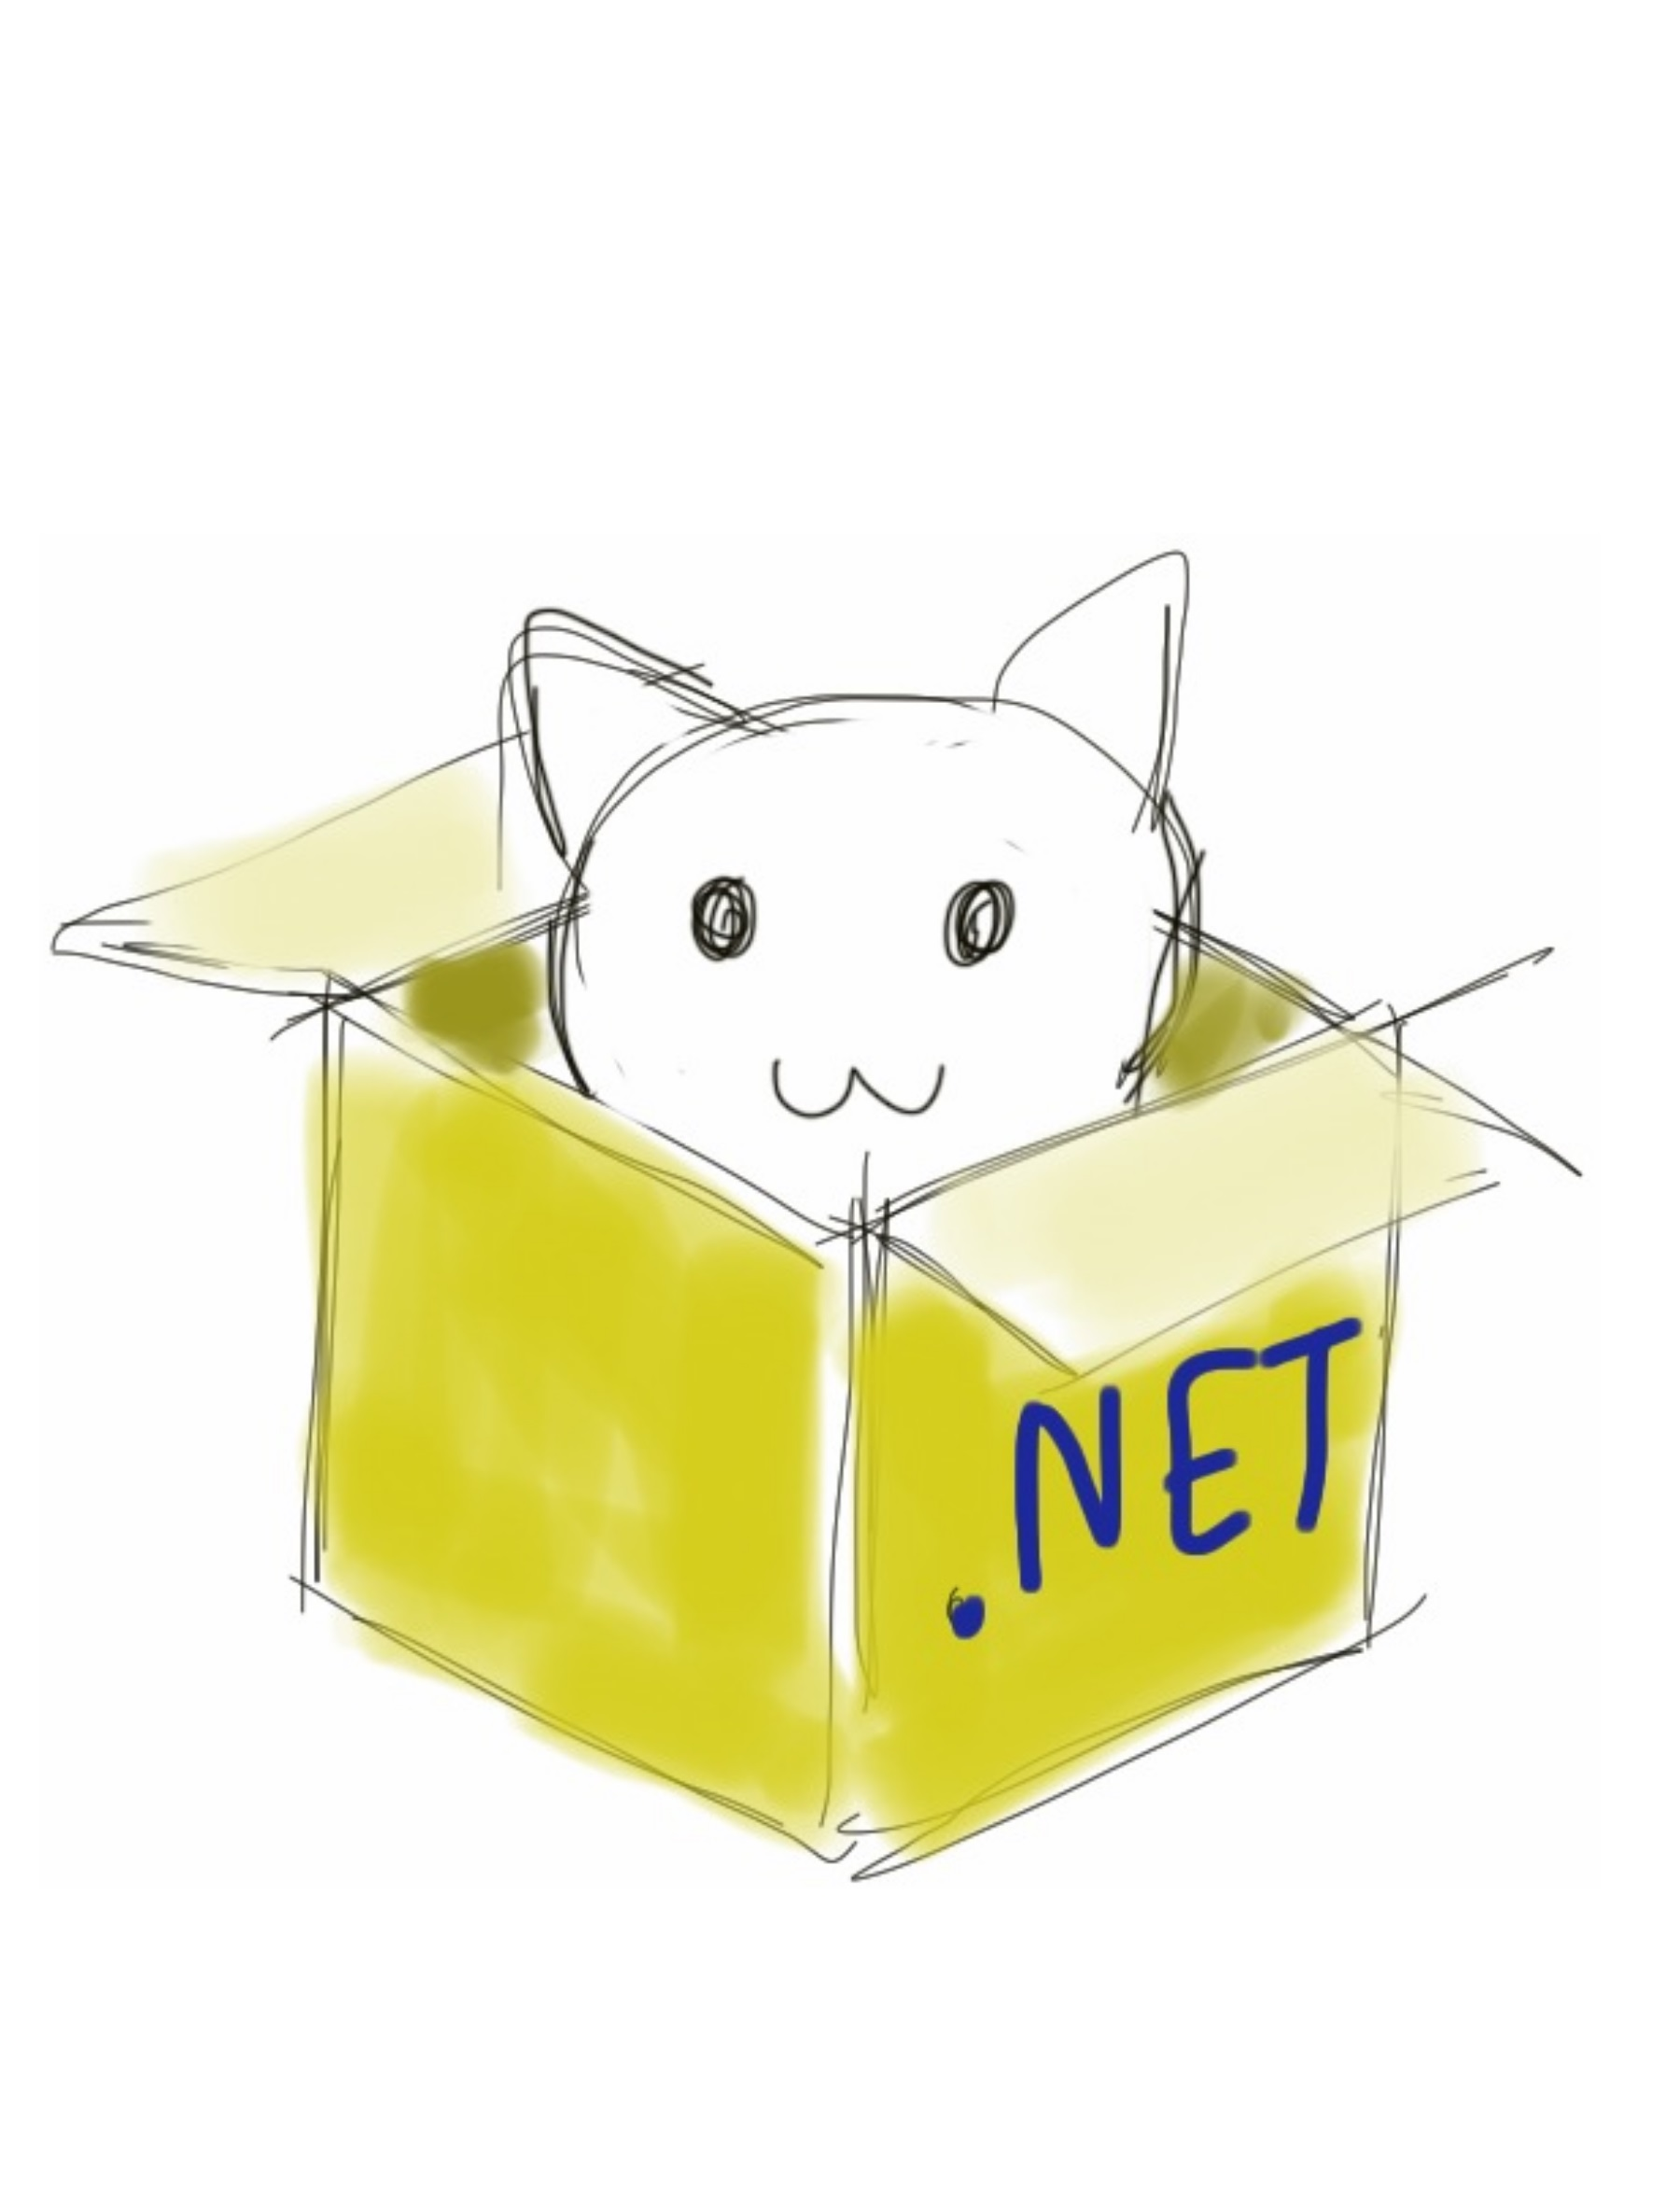
\includegraphics[width=0.8\textwidth]{cover}
\end{center}
\newpage

%%%%%%%%%%%%%%%%%%%% Copyright page %%%%%%%%%%%%%%%%%%%%
\hbox{}
\vfill
{
\noindent
«Задачник.NET»\\
\copyright\ 2014, Андрей Акиньшин <\href{mailto:andrey.akinshin@gmail.com}{andrey.akinshin@gmail.com}>\\
Под редакцией Ивана Пащенко\\
% DOI: \href{http://dx.doi.org/10.5281/zenodo.11839}{10.5281/zenodo.11839}

\medskip
\noindent
Это произведение доступно по лицензии Creative Commons «Attribution-NonCommercial-NoDerivatives» («Атрибуция — Некоммерческое использование — Без производных произведений») 4.0 Всемирная. Чтобы увидеть копию этой лицензии, посетите:\\ \url{http://creativecommons.org/licenses/by-nc-nd/4.0/}.\\
Версия текста: v-\versiondate\today \newline
Исходные коды и актуальная версия текст доступны по адресу:\\ \url{https://github.com/AndreyAkinshin/ProblemBook.NET}
}
\newpage